\clearpage % Rozdziały zaczynamy od nowej strony.

\section{Testowanie systemu}

Aby zapewnić najwyższą jakość tworzonego oprogramowania, kluczowe jest włączenie etapu testowania do procesu jego rozwoju. Celem testowania jest identyfikacja i eliminacja błędów, zazwyczaj przed oficjalnym wdrożeniem produktu. W tym procesie stosuje się różnorodne metody i narzędzia. We wdrożonym systemie, zostały wykorzystane cztery główne rodzaje testów: testy jednostkowe, które koncentrują się na najmniejszych częściach kodu; testy integracyjne, sprawdzające współdziałanie poszczególnych modułów; testy akceptacyjne, które oceniają oprogramowanie z perspektywy użytkownika końcowego oraz testy wydajnościowe, mające na celu ocenę szybkości i stabilności działania systemu.

\subsection{Testy jednostkowe}

Testy jednostkowe są najmniejszymi testami, które można przeprowadzić na oprogramowaniu. Ich celem jest sprawdzenie, czy najmniejsze części kodu, np. pojedyncze funkcje, klasy, działają poprawnie. W ramach pracy inżynierskiej testy jednostkowe zostały przeprowadzone przy pomocy narzędzia Kotest \cite{kotest} oraz pakietu \textit{org.axonframework:axon-test} pomocniczego w testowaniu aplikacji opartych na frameworku Axon.

Pokrycie kodu reprezentowane jest przez procentowy udział linii kodu, które zostały przetestowane. W ramach pracy inżynierskiej, pokrycie kodu zostało zmierzone przy pomocy narzędzia JaCoCo \cite{jacoco}. Cel pokrycia kodu został ustalony na poziomie 80\%. W implementowanym systemie, pokrycie całego kodu wyniosło 83\%, a pokrycie kodu warstwy dziedziny wyniosło 100\%.

\begin{lstlisting}[caption={Przykładowy test jednostkowy serwisu zamówień},label={lst:testing-unit},captionpos=b,language=Kotlin,numbers=left]
class OrderTest {

    private lateinit var testFixture: AggregateTestFixture<Order>
    private lateinit var orderVerificationPort: OrderVerificationPort

    @BeforeEach
    fun setUp() {
        orderVerificationPort = mockk<OrderVerificationPort>()
        testFixture = AggregateTestFixture(Order::class.java)
        testFixture.registerInjectableResource(orderVerificationPort)
    }

    @Test
    fun `given created order, should finalize order`() {
        val orderStartedEvent = OrderStartedEvent(
            orderId = UUID.randomUUID(),
            userId = "user",
            restaurantId = UUID.randomUUID(),
            status = OrderStartedEvent.OrderStatus.CREATED
        )

        val orderItemAddedEvent = OrderItemAddedEvent(
            orderId = orderStartedEvent.orderId,
            productId = UUID.randomUUID()
        )

        val finalizeOrderCommand = FinalizeOrderCommand(
            orderId = orderStartedEvent.orderId,
            userId = orderStartedEvent.userId
        )

        every {
            orderVerificationPort.productExists(
                orderItemAddedEvent.productId,
                orderStartedEvent.restaurantId
            )
        } returns true

        val orderFinalizedEvent = OrderFinalizedEvent(
            orderId = orderStartedEvent.orderId,
            userId = orderStartedEvent.userId,
            restaurantId = orderStartedEvent.restaurantId,
            items = mapOf(orderItemAddedEvent.productId to 1)
        )

        testFixture.given(orderStartedEvent, orderItemAddedEvent)
            .`when`(finalizeOrderCommand)
            .expectSuccessfulHandlerExecution()
            .expectEvents(orderFinalizedEvent)
    }
}
\end{lstlisting}

Na wycinku \ref{lst:testing-unit} przedstawiono przykładowy test jednostkowy serwisu zamówień, weryfikujący zachowanie agregatu dla komendy finalizującej zamówienie. W liniach 6-11 przedstawiono przygotowanie testu, polegające na utworzeniu obiektu testowego oraz zarejestrowaniu w nim testowej implementacji portu weryfikacji zamówień. W liniach 13-51 przedstawiono scenariusz testowy, polegający na wywołaniu komendy finalizującej zamówienie, a następnie sprawdzeniu, czy agregat wyemitował oczekiwane zdarzenie.

Dzięki pakietowi pomocniczemu frameworka Axon takie testy są łatwe w implementacji i dalszym utrzymaniu. Dzięki zastosowaniu technik DDD oraz Event Sourcing możliwe jest przetestowanie zachowania logiki biznesowej bez konieczności uruchamiania całej aplikacji, przez co wykonywanie takich testów jest szybkie i wydajne.

\subsection{Testy integracyjne}

Testy integracyjne sprawdzają współdziałanie poszczególnych modułów systemu. W ramach pracy inżynierskiej testy jednostkowe zostały przeprowadzone przy pomocy tych samych narzędzi co jednostkowe, z dodatkową pomocą biblioteki \linebreak \textit{org.springframework.boot:spring-boot-starter-test}, pozwalającej na uruchomienie testów w kontekście aplikacji Spring Boot.

W celu przygotowania środowiska testowego należy uruchomić lokalnie instancję Axon Server np. przy pomocy Dockera \cite{docker}.

\begin{lstlisting}[caption={Przykładowy test integracyjny serwisu zamówień},label={lst:testing-integration},captionpos=b,language=Kotlin,numbers=left]
@SpringBootTest
@ActiveProfiles("test")
class OrderTestIT {

    @Autowired
    private lateinit var commandGateway: CommandGateway

    @Autowired
    private lateinit var aggregateRepository: Repository<Order>

    @Test
    fun `given open restaurant and user, should start order`() {
        val orderId = commandGateway.sendAndWait<UUID>(
            StartOrderCommand(
                orderId = UUID.randomUUID(),
                userId = "userId",
                restaurantId = UUID.randomUUID()
            )
        )

        val order = aggregateRepository.load(orderId.toString())
        order.userId shouldBe "userId"
    }
}
\end{lstlisting}

Na wycinku \ref{lst:testing-integration} przedstawiono przykładowy test integracyjny serwisu zamówień, weryfikujący, że po wysłaniu komendy rozpoczęcia zamówienia, agregat został poprawnie utworzony. W przeciwieństwie do testów jednostkowych test ten weryfikuje również działanie komponentów odpowiedzialnych za przesyłanie komend do agregatów oraz zapisywanie zdarzeń do magazynu zdarzeń. Testy te są bardziej złożone w implementacji, ale pozwalają na weryfikację działania całego systemu.

\subsection{Testy akceptacyjne}

Testy akceptacyjne sprawdzają, czy system spełnia wymagania użytkownika końcowego. W ramach pracy inżynierskiej testy akceptacyjne zostały przeprowadzone przy pomocy narzędzia RestAssured \cite{restassured}, które pozwala na testowanie interfejsu REST API. Zaimplementowano jeden scenariusz testowy, który przechodzi przez wszystkie funkcjonalności systemu, od rejestracji użytkownika, przez dodanie restauracji, złożenie zamówienia, aż do jego dostarczenia.

Służy on również jako weryfikacja poprawnego działania systemu po wdrożeniu nowej wersji w ramach potoku CI/CD.

\begin{lstlisting}[caption={Scenariusz testowy w ramach testów akceptacyjnych},label={lst:testing-acceptance},captionpos=b,language=Kotlin,numbers=left]
@Test
fun e2e() {
    // setup
    setupRestaurant()
    setupOrderingUser()
    setupCourier()

    // user
    createOrder()
    payOrder()

    // restaurant
    acceptRestaurantOrder()
    prepareRestaurantOrder()

    // courier
    acceptDeliveryOffer()
    pickupDelivery()
    deliverDelivery()

    // payments
    withdrawRestaurantBalance()
    withdrawCourierBalance()
}
\end{lstlisting}

Na wycinku \ref{lst:testing-acceptance} przedstawiono jedynie fragment wspomnianego testu, ze względu na jego długość. Test ten weryfikuje, czy system spełnia wymagania użytkownika końcowego, a także czy wszystkie komponenty współpracują ze sobą poprawnie. Test ten jest bardzo złożony w implementacji, ale pozwala na weryfikację działania całego systemu.

Weryfikuje on również integrację z zewnętrznymi systemami, takimi jak system płatności Stripe, poprzez wykorzystanie biblioteki Selenium \cite{selenium}, umożliwiającej automatyzację przeglądarek internetowych, co pozwala na manualne przejście procesu płatności.

\subsection{Testy wydajnościowe}

Testy wydajnościowe mają na celu ocenę szybkości i stabilności działania systemu. Pozwalają one przewidywać zachowanie systemu pod wzrastającym obciążeniem, umożliwiając zaplanowanie odpowiednich ulepszeń infrastruktury i kodu.

W ramach pracy inżynierskiej przeprowadzono testy wydajnościowe przy pomocy narzędzia Locust \cite{locust} w języku Python. Narzędzie to pozwala na symulację wielu użytkowników, którzy wykonują określone akcje w systemie. Przeprowadzono testy z perspektywy trzech rodzajów użytkowników: użytkownika zamawiającego, managera restauracji oraz kuriera. Każdy rodzaj użytkownika został zdefiniowany przez klasę w języku Python, która implementuje logikę wykonywania akcji w systemie. 

Przykład scenariusza testowego został przedstawiony na wycinku \ref{lst:testing-performance}.

\begin{lstlisting}[caption={Scenariusz testowy w ramach testów wydajnościowych obsługujących managera restauracji},label={lst:testing-performance},captionpos=b,language=Python,numbers=left]
class RestaurantManager(HttpUser):
    def on_start(self):
        self.client.headers["X-User-Id"] = fake.uuid4()
        self._create_restaurant()

    @task
    def e2e(self):
        restaurant_orders = self.client.get(
            f"/v2/restaurants/{self.restaurant_id}/orders"
        ).json()

        selected_order = random.choice(restaurant_orders)
        restaurant_order_id = selected_order.get("restaurantOrderId")

        self.client.put(f"/v1/orders/{restaurant_order_id}/accept")

        self.client.put(f"/v1/orders/{restaurant_order_id}/prepare" )
\end{lstlisting}

Klasa ta imituje zachowanie managera restauracji, który po zalogowaniu się do systemu, pobiera listę zamówień, wybiera jedno z nich, a następnie akceptuje i przygotowuje je do dostarczenia.

W ramach testów wydajnościowych przeprowadzono testy z perspektywy 100, 200, 300, 500 i 1000 użytkowników. Wszystkie testy zostały wykonane na lokalnym środowisku, przy pomocy trzech instancji narzędzia Locust. Wszystkie testy zostały przeprowadzone na wdrożonej w chmurowym klastrze Kubernetes produkcyjnej wersji systemu, bez żadnych dodatkowych optymalizacji. Klaster skonfigurowano z trzema węzłami typu \textit{e2-standard-4}, jak opisano w rozdziale dotyczącym wdrożenia. Każdy serwis systemu został uruchomiony w czterech instancjach. Liczba użytkowników była zwiększana stopniowo, po 5 użytkowników na sekundę, aż do osiągnięcia docelowej liczby użytkowników. Rezultaty testów były zapisywane po dziesięciu minutach od rozpoczęcia testu. 

Wyniki testów wydajnościowych zostały przedstawione w tabeli \ref{table:performance}. Śledzonymi metrykami były liczba żądań na sekundę, średnie czasy odpowiedzi oraz opóźnienie obsługi zdarzeń. Opóźnienie obsługi zdarzeń to czas, który upłynął od momentu wygenerowania zdarzenia przez system, do momentu jego obsłużenia przez wszystkie komponenty systemu.

\begin{longtable}{| m{0.25\linewidth} | m{0.2\linewidth} | m{0.25\linewidth} | m{0.2\linewidth} |}
    \caption{Rezultaty testów wydajnościowych}
    \label{table:performance} \\

    \hline
    Liczba użytkowników & Liczba żądań na sekundę & Czasy odpowiedzi & Opóźnienie obsługi zdarzeń \\ \hline\hline \endfirsthead \endfoot
    \hline \endlastfoot

    100 & 90,5 & Percentyl 50\% - 13 ms \newline Percentyl 95\% - 24 ms & 3 ms \\ \hline
    200 & 183,2 & Percentyl 50\% - 15 ms \newline Percentyl 95\% - 29 ms & 10 ms \\ \hline
    300 & 264,7 & Percentyl 50\% - 16 ms \newline Percentyl 95\% - 30 ms & 6 ms \\ \hline
    500 & 438,1 & Percentyl 50\% - 59 ms \newline Percentyl 95\% - 210 ms & 8,86 s \\ \hline
    1000 & 886,2 & Percentyl 50\% - 62 ms \newline Percentyl 95\% - 160 ms & 16,12 s \\ \hline
\end{longtable}

System zachowywał się stabilnie do momentu osiągnięcia liczby 500 użytkowników. W tym momencie, opóźnienie obsługi zdarzeń zaczęło gwałtownie rosnąć, co oznacza, że system nie był w stanie obsłużyć wszystkich zdarzeń w czasie rzeczywistym. Jednocześnie, nadal obsługiwał on wszystkie żądania w akceptowalnym czasie. Problem z opóźnieniem obsługi zdarzeń rósł wraz ze wzrostem liczby użytkowników. W przypadku 1000 użytkowników, opóźnienie obsługi zdarzeń wyniosło 16,12 sekundy.


Na rysunku \ref{fig:locust} przedstawiono przykładowy rezultat wykonania testów wydajnościowych. Na wykresie przedstawiono liczbę użytkowników, którzy wykonują akcje w systemie, liczbę zapytań na sekundę, które są wykonywane oraz średnie czasy odpowiedzi.

\begin{figure}[!h]
    \centering 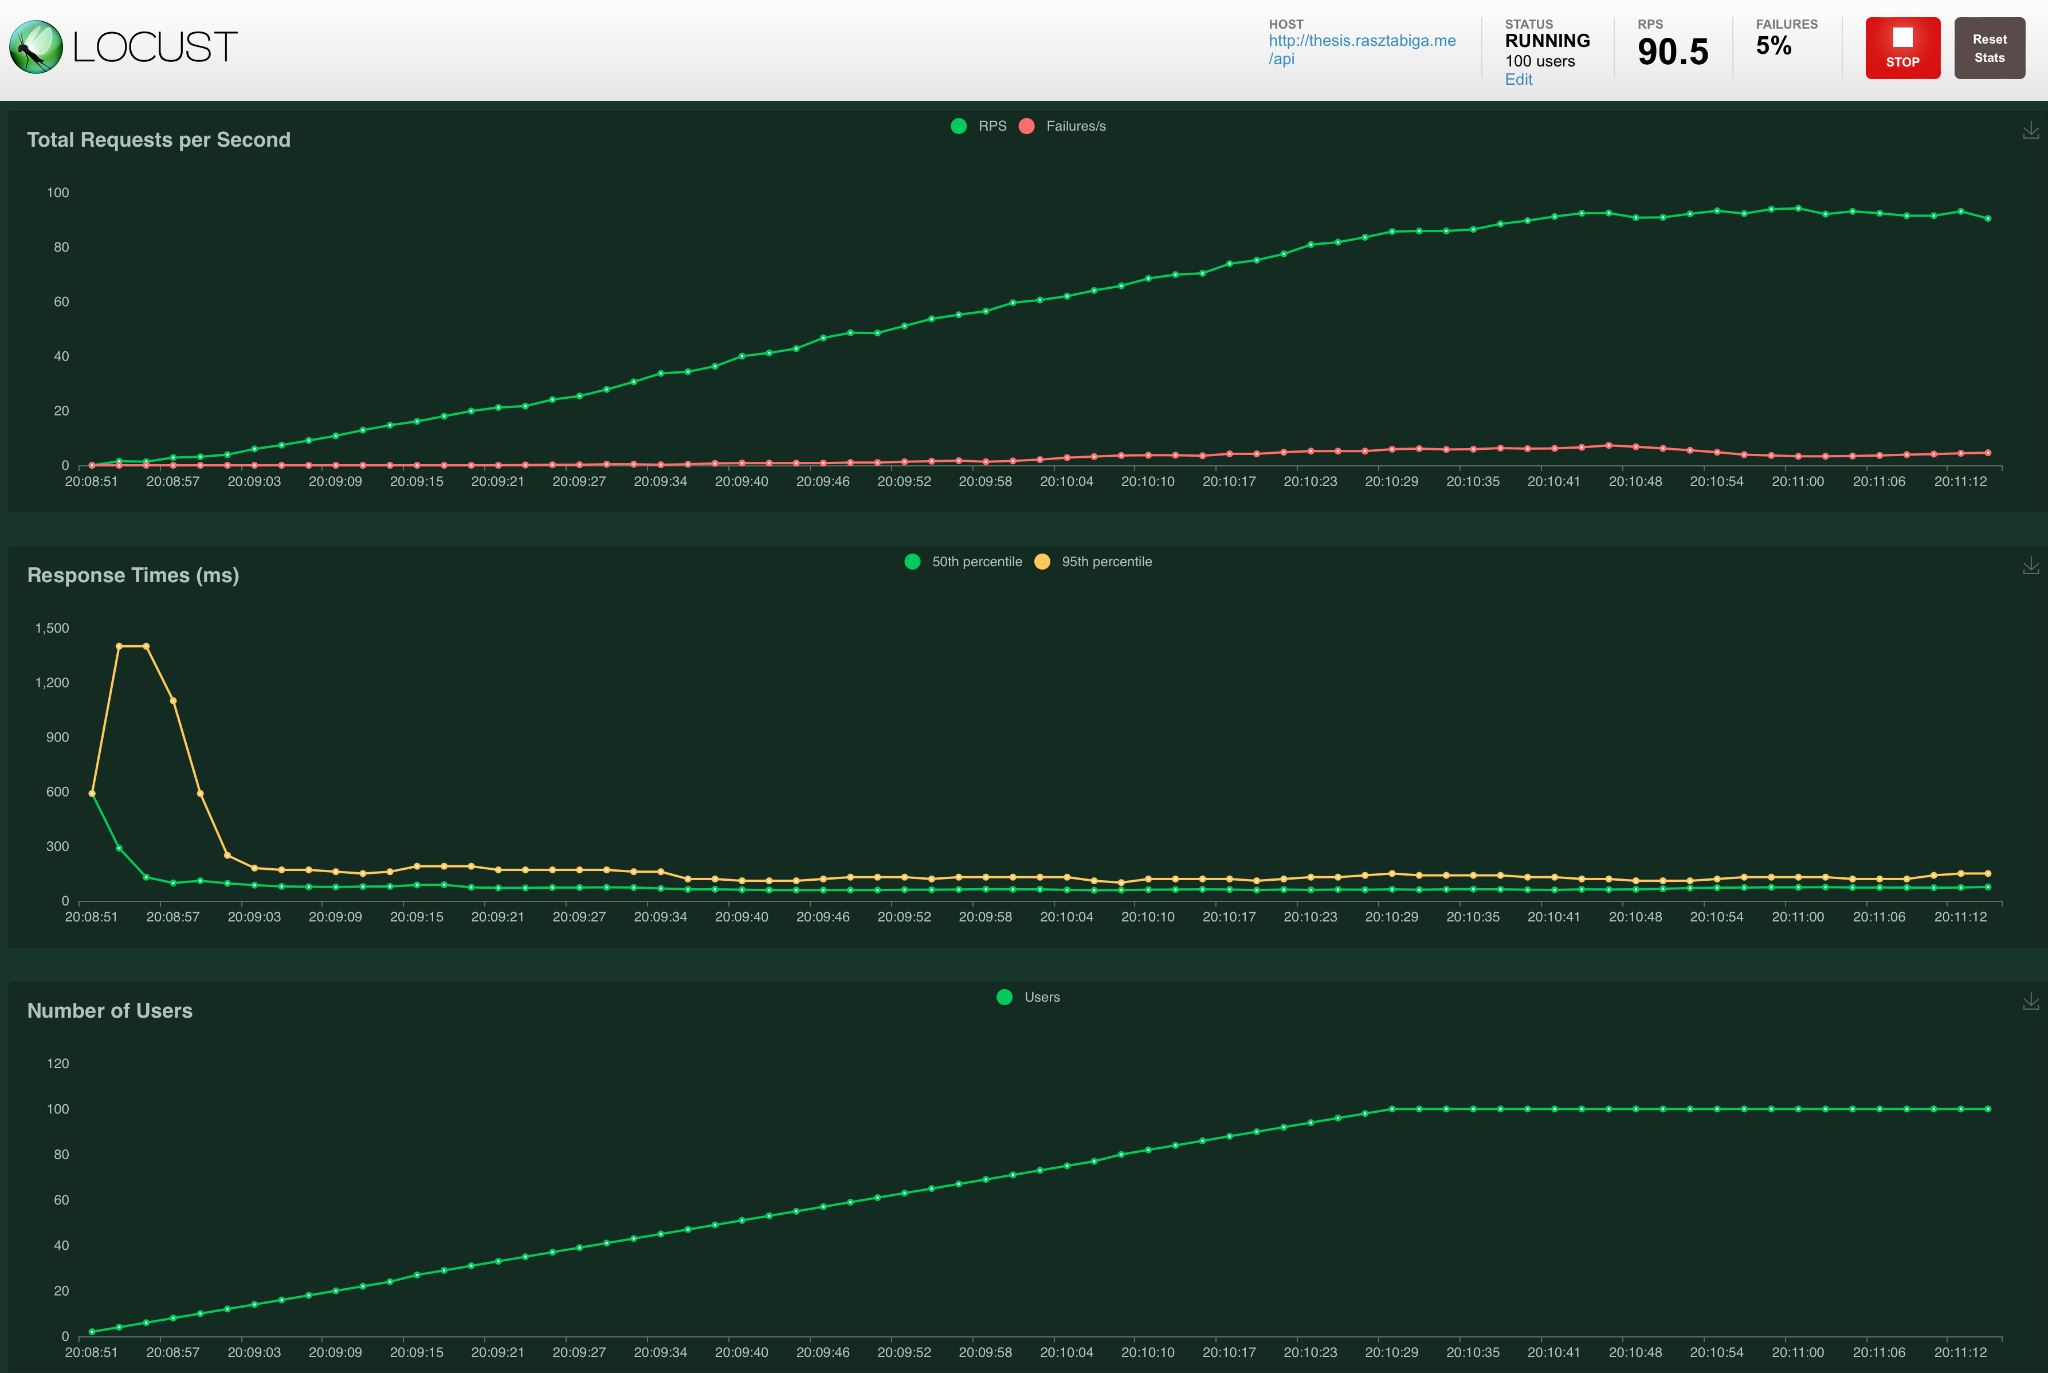
\includegraphics[width=1.0\linewidth]{locust.png}
    \caption{Przykładowy rezultat wykonania testów wydajnościowych}
    \label{fig:locust}
\end{figure}